The algorithm above shows that, if $\tilde R_n = \rank(\St_{([n])})$ for all $n$, then there exists a TT decomposition of rank-$(\tilde R_1,\dots, \tilde R_{N-1})$, showing that the TT rank $(R_1,\dots, R_{N-1})$ of $\St$ is upper-bounded by the rank of the matricizations: $ R_n \leq \rank(\St_{([n])} )$ for all $n$. It is also easy to show that the TT rank is lower-bounded by the rank of the matricizations. Indeed, suppose that $\St$ has the TT rank  $(R_1,\dots, R_{N-1})$. Then, there exists a rank-$(R_1,\dots, R_{N-1})$ TT decomposition. Using Theorem~\ref{thm: matricization-rank}, we can easily see that this implies $\rank(\St_{([n])} )\leq  R_n$ for all $n$.
\end{proof}
Although the proof above uses successive QR decompositions to construct an exact TT decomposition, the algorithm commonly referred to as TT-SVD uses SVDs of the successive unfoldings. In the exact case, retaining all nonzero singular values yields TT ranks
$
R_n = \rank(\St_{([n])} )
$.
The advantage of the SVD formulation is that it immediately provides a low-rank approximation algorithm: at each step, truncated SVD can be used to prescribed TT ranks or according to a tolerance on the discarded singular values~\citep{oseledets2010approximation,holtz2012manifolds}.

Another widely used approach for decomposing a tensor into the tensor-train (TT) format is the Alternating Least Squares (ALS) algorithm. Before introducing this method, we first describe the canonical form of the TT decomposition.
\begin{definition}\label{def:canonical-form}
   The TT decomposition $\TT(({\At_n})_{n=1}^N)\in\RR^{d_1\times\dots\times d_N}$ is said to be in canonical form with respect to a fixed index $j\in [N]$ if all cores with $n<j$ are left-orthogonal and all cores with $n>j$ are right-orthogonal, e.g., the following TT decomposition is in canonical form with respect to its third core tensor:
$$
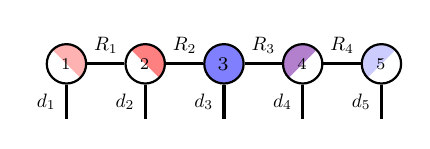
\begin{tikzpicture}[baseline=-0.5ex]
    \tikzset{tensor/.style = {minimum size = 0.5cm,shape = circle,thick,draw=black,inner sep = 0pt}, edge/.style = {thick,line width=.4mm},every loop/.style={}}
    \def\x{0}
    \def\y{0}
 \node[tensor, path picture={
        \fill[fill=red!30!white](path picture bounding box.south east)
        -- 
        (path picture bounding box.north west) --
        (path picture bounding box.north east) -- cycle;
        }, shift={(\x,\y)}] (A) {\scalebox{0.85}{$\At_1$}};
        \draw[edge](A) -- (\x,\y-0.7) node [midway,left] {\scalebox{0.7}{\dimcolor{$d_1$}}};
       \node[tensor, path picture={
        \fill[fill=red!50!white](path picture bounding box.south east)
        -- 
        (path picture bounding box.north west) --
        (path picture bounding box.north east) -- cycle;
        }, shift={(\x+1,\y)}] (B) {\scalebox{0.85}{$\At_2$}};
         \draw[edge](B) -- (\x+1,\y-0.7)node [midway,left] {\scalebox{0.7}{\dimcolor{$d_2$}}};
         \node[tensor,fill=blue!50!white] (C) at (\x+2,\y){$\At_3$};
          \draw[edge](C) -- (\x+2,\y-0.7)node [midway,left] {\scalebox{0.7}{\dimcolor{$d_3$}}};
          \node[tensor, path picture={
        \fill[fill=blue!60!red!50!](path picture bounding box.south west)
        -- 
        (path picture bounding box.north east) --
        (path picture bounding box.north west) -- cycle;
        }, shift={(\x+3,\y)}] (D) {\scalebox{0.85}{$\At_4$}};
         \draw[edge](D) -- (\x+3,\y-0.7)node [midway,left] {\scalebox{0.7}{\dimcolor{$d_4$}}};
           \node[tensor, path picture={
        \fill[fill=blue!20!white](path picture bounding box.south west)
        -- 
        (path picture bounding box.north east) --
        (path picture bounding box.north west) -- cycle;
        }, shift={(\x+4,\y)}] (E) {\scalebox{0.85}{$\At_5$}};
         \draw[edge](E) -- (\x+4,\y-0.7)node [midway,left] {\scalebox{0.7}{\dimcolor{$d_5$}}};
    \draw[edge](A) -- (B) node [midway,above] {\scalebox{0.7}{\dimcolor{$R_1$}}};
    \draw[edge](B) -- (C) node [midway,above] {\scalebox{0.7}{\dimcolor{$R_2$}}};
    \draw[edge](C) -- (D) node [midway,above] {\scalebox{0.7}{\dimcolor{$R_3$}}};
    \draw[edge](D) -- (E) node [midway,above] {\scalebox{0.7}{\dimcolor{$R_4$}}};
\end{tikzpicture}.
$$
The cores on the left side of $\At_3$ are left-orthogonal and the cores on the right are right-orthogonal. The core $\At_3$ is called the center of  orthogonality. Note that any TT decomposition can be efficiently converted to a canonical form w.r.t. any index $j\in [N]$ by performing a series of QR decompositions on the core tensors~\citep{holtz2012alternating,evenbly2018gauge}.
\end{definition}
\paragraph{Computing TT with Alternating Least Squares~(ALS)} The single-site Tensor Train Alternating Least Squares (TT-ALS) method~\citep{holtz2012alternating} starts with a TT decomposition in canonical form, initialized with a crude approximation~(e.g., with random cores, or using TT-SVD).
In the first step, the core 
$\At_1$ of the decomposition is non-orthogonal. During sweeps from left to right~(respectively, right to left), the algorithm keeps all cores fixed except for the $n$-th  one, $\At_n$, and optimizes it to minimize the distance to the target tensor. The resulting minimization problem is a simple least-squares problem, hence the name  ALS.  
After updating $\At_n$, a QR decomposition is applied to ensure numerical stability and to maintain the canonical form. The non-orthonormal factor is then merged into the left (or right, depending on the sweep direction), a step known as \textit{core orthogonalization}.
\begin{figure}[h!]
    \centering
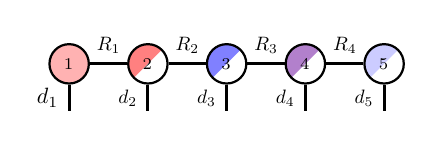
\begin{tikzpicture}[baseline=-0.5ex]
    \tikzset{tensor/.style = {minimum size = 0.5cm,shape = circle,thick,draw=black,inner sep = 0pt}, edge/.style = {thick,line width=.4mm},every loop/.style={}}
    \def\x{0}
    \def\y{0}
    \node[tensor, 
        fill=red!30!white, shift = {(\x-4,\y)}] (A) {\scalebox{0.85}{$\At_1$}};
        \draw[edge](A) -- (\x-4,\y-0.6) node [midway,left] {\scalebox{0.8}{\dimcolor{$d_1$}}};
       \node[tensor, path picture={
        \fill[fill=red!50!white](path picture bounding box.south west)
        -- 
        (path picture bounding box.north east) --
        (path picture bounding box.north west) -- cycle;
        }, shift={(\x-3,\y)}] (B) {\scalebox{0.85}{$\At_2$}};
       \draw[edge](B) -- (\x-3,\y-0.6)node [midway,left] {\scalebox{0.7}{\dimcolor{$d_2$}}};
        \node[tensor, path picture={
        \fill[fill=blue!50!white](path picture bounding box.south west)
        -- 
        (path picture bounding box.north east) --
        (path picture bounding box.north west) -- cycle;
        }, shift={(\x-2,\y)}] (C) {\scalebox{0.85}{$\At_3$}};
        \draw[edge](C) -- (\x-2,\y-0.6)node [midway,left] {\scalebox{0.7}{\dimcolor{$d_3$}}};
        \node[tensor, path picture={
       \fill[fill=blue!60!red!50!](path             picture bounding box.south west)
        -- 
        (path picture bounding box.north east) --
       (path picture bounding box.north west) -- cycle;}, shift={(\x-1,\y)}] (D) {\scalebox{0.85}{$\At_4$}};
    \draw[edge](D) -- (\x-1,\y-0.6)node [midway,left] {\scalebox{0.7}{\dimcolor{$d_4$}}};
    \node[tensor, path picture={
    \fill[fill= blue!20!white](path             picture bounding box.south west)
    -- 
    (path picture bounding box.north east) --
    (path picture bounding box.north west) -- cycle;}, shift={(\x,\y)}] (E) {\scalebox{0.85}{$\At_5$}};
    \draw[edge](E) -- (\x,\y-0.6)node [midway,left] {\scalebox{0.7}{\dimcolor{$d_5$}}};
    \draw[edge](A) -- (B) node [midway,above] {\scalebox{0.7}{\dimcolor{$R_1$}}};
    \draw[edge](B) -- (C) node [midway,above] {\scalebox{0.7}{\dimcolor{$R_2$}}};
    \draw[edge](C) -- (D) node [midway,above] {\scalebox{0.7}{\dimcolor{$R_3$}}};
    \draw[edge](D) -- (E) node [midway,above] {\scalebox{0.7}{\dimcolor{$R_4$}}};
\end{tikzpicture}~~~\text{step:~1}\\
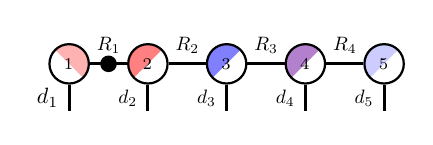
\begin{tikzpicture}[baseline=-0.5ex]
    \tikzset{tensor/.style = {minimum size = 0.5cm,shape = circle,thick,draw=black,inner sep = 0pt}, edge/.style = {thick,line width=.4mm},every loop/.style={}}
    \def\x{0}
    \def\y{0}
    \node[tensor, path picture = {
        \fill[fill=red!30!white] (path picture bounding box.south east)
        -- 
        (path picture bounding box.north west) --
        (path picture bounding box.north east) -- cycle;
        }, shift = {(\x-4,\y)}] (A) {\scalebox{0.85}{$\At_1$}};
        \draw[edge](A) -- (\x-4,\y-0.6) node [midway,left] {\scalebox{0.8}{\dimcolor{$d_1$}}};
         \draw  node[fill = black,circle,inner sep=0pt,minimum size=6pt] (m) at (\x-3.5,\y) {};
       \node[tensor, path picture={
        \fill[fill=red!50!white](path picture bounding box.south west)
        -- 
        (path picture bounding box.north east) --
        (path picture bounding box.north west) -- cycle;
        }, shift={(\x-3,\y)}] (B) {\scalebox{0.85}{$\At_2$}};
       \draw[edge](B) -- (\x-3,\y-0.6)node [midway,left] {\scalebox{0.7}{\dimcolor{$d_2$}}};
        \node[tensor, path picture={
        \fill[fill=blue!50!white](path picture bounding box.south west)
        -- 
        (path picture bounding box.north east) --
        (path picture bounding box.north west) -- cycle;
        }, shift={(\x-2,\y)}] (C) {\scalebox{0.85}{$\At_3$}};
        \draw[edge](C) -- (\x-2,\y-0.6)node [midway,left] {\scalebox{0.7}{\dimcolor{$d_3$}}};
        \node[tensor, path picture={
       \fill[fill=blue!60!red!50!](path             picture bounding box.south west)
        -- 
        (path picture bounding box.north east) --
       (path picture bounding box.north west) -- cycle;}, shift={(\x-1,\y)}] (D) {\scalebox{0.85}{$\At_4$}};
    \draw[edge](D) -- (\x-1,\y-0.6)node [midway,left] {\scalebox{0.7}{\dimcolor{$d_4$}}};
    \node[tensor, path picture={
    \fill[fill= blue!20!white](path             picture bounding box.south west)
    -- 
    (path picture bounding box.north east) --
    (path picture bounding box.north west) -- cycle;}, shift={(\x,\y)}] (E) {\scalebox{0.85}{$\At_5$}};
    \draw[edge](E) -- (\x,\y-0.6)node [midway,left] {\scalebox{0.7}{\dimcolor{$d_5$}}};
    \draw[edge](A) -- (B) node [midway,above] {\scalebox{0.7}{\dimcolor{$R_1$}}};
    \draw[edge](B) -- (C) node [midway,above] {\scalebox{0.7}{\dimcolor{$R_2$}}};
    \draw[edge](C) -- (D) node [midway,above] {\scalebox{0.7}{\dimcolor{$R_3$}}};
    \draw[edge](D) -- (E) node [midway,above] {\scalebox{0.7}{\dimcolor{$R_4$}}};
\end{tikzpicture}~~~~~~\text{QR}\\
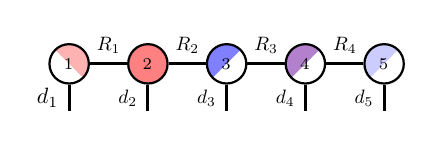
\begin{tikzpicture}[baseline=-0.5ex]
    \tikzset{tensor/.style = {minimum size = 0.5cm,shape = circle,thick,draw=black,inner sep = 0pt}, edge/.style = {thick,line width=.4mm},every loop/.style={}}
    \def\x{0}
    \def\y{0}
    \node[tensor, path picture = {
        \fill[fill=red!30!white] (path picture bounding box.south east)
        -- 
        (path picture bounding box.north west) --
        (path picture bounding box.north east) -- cycle;
        }, shift = {(\x-4,\y)}] (A) {\scalebox{0.85}{$\At_1$}};
        \draw[edge](A) -- (\x-4,\y-0.6) node [midway,left] {\scalebox{0.8}{\dimcolor{$d_1$}}};
       \node[tensor, 
        fill=red!50!white, shift = {(\x-3,\y)}] (B) {\scalebox{0.85}{$\At_2$}};
       \draw[edge](B) -- (\x-3,\y-0.6)node [midway,left] {\scalebox{0.7}{\dimcolor{$d_2$}}};
        \node[tensor, path picture={
        \fill[fill=blue!50!white](path picture bounding box.south west)
        -- 
        (path picture bounding box.north east) --
        (path picture bounding box.north west) -- cycle;
        }, shift={(\x-2,\y)}] (C) {\scalebox{0.85}{$\At_3$}};
        \draw[edge](C) -- (\x-2,\y-0.6)node [midway,left] {\scalebox{0.7}{\dimcolor{$d_3$}}};
        \node[tensor, path picture={
       \fill[fill=blue!60!red!50!](path             picture bounding box.south west) -- (path picture bounding box.north east) -- (path picture bounding box.north west) -- cycle;}, shift={(\x-1,\y)}] (D) {\scalebox{0.85}{$\At_4$}};
    \draw[edge](D) -- (\x-1,\y-0.6)node [midway,left] {\scalebox{0.7}{\dimcolor{$d_4$}}};
    \node[tensor, path picture={
    \fill[fill= blue!20!white](path picture bounding box.south west)
    -- 
    (path picture bounding box.north east) --
    (path picture bounding box.north west) -- cycle;}, shift={(\x,\y)}] (E) {\scalebox{0.85}{$\At_5$}};
    \draw[edge](E) -- (\x,\y-0.6)node [midway,left] {\scalebox{0.7}{\dimcolor{$d_5$}}};
    \draw[edge](A) -- (B) node [midway,above] {\scalebox{0.7}{\dimcolor{$R_1$}}};
    \draw[edge](B) -- (C) node [midway,above] {\scalebox{0.7}{\dimcolor{$R_2$}}};
    \draw[edge](C) -- (D) node [midway,above] {\scalebox{0.7}{\dimcolor{$R_3$}}};
    \draw[edge](D) -- (E) node [midway,above] {\scalebox{0.7}{\dimcolor{$R_4$}}};
\end{tikzpicture}~~~\text{step:~2}\\
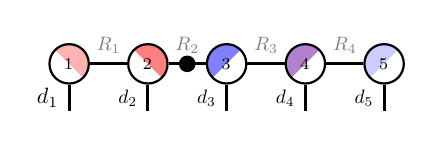
\begin{tikzpicture}[baseline=-0.5ex]
    \tikzset{tensor/.style = {minimum size = 0.5cm,shape = circle,thick,draw=black,inner sep = 0pt}, edge/.style = {thick,line width=.4mm},every loop/.style={}}
    \def\x{0}
    \def\y{0}
    \node[tensor, path picture = {
        \fill[fill=red!30!white] (path picture bounding box.south east)
        -- 
        (path picture bounding box.north west) --
        (path picture bounding box.north east) -- cycle;
        }, shift = {(\x-4,\y)}] (A) {\scalebox{0.85}{$\At_1$}};
        \draw[edge](A) -- (\x-4,\y-0.6) node [midway,left] {\scalebox{0.8}{\dimcolor{$d_1$}}};
       \node[tensor, path picture={
        \fill[fill=red!50!white](path picture bounding box.south east)
        -- 
        (path picture bounding box.north west) --
        (path picture bounding box.north east) -- cycle;
        }, shift={(\x-3,\y)}] (B) {\scalebox{0.85}{$\At_2$}};
       \draw[edge](B) -- (\x-3,\y-0.6)node [midway,left] {\scalebox{0.7}{\dimcolor{$d_2$}}};
        \draw  node[fill = black,circle,inner sep=0pt,minimum size=6pt] (m) at (\x-2.5,\y) {};
        \node[tensor, path picture={
        \fill[fill=blue!50!white](path picture bounding box.south west)
        -- 
        (path picture bounding box.north east) --
        (path picture bounding box.north west) -- cycle;
        }, shift={(\x-2,\y)}] (C) {\scalebox{0.85}{$\At_3$}};
        \draw[edge](C) -- (\x-2,\y-0.6)node [midway,left] {\scalebox{0.7}{\dimcolor{$d_3$}}};
        \node[tensor, path picture={
       \fill[fill=blue!60!red!50!](path             picture bounding box.south west)
        -- 
        (path picture bounding box.north east) --
       (path picture bounding box.north west) -- cycle;}, shift={(\x-1,\y)}] (D) {\scalebox{0.85}{$\At_4$}};
    \draw[edge](D) -- (\x-1,\y-0.6)node [midway,left] {\scalebox{0.7}{\dimcolor{$d_4$}}};
    \node[tensor, path picture={
    \fill[fill= blue!20!white](path             picture bounding box.south west)
    -- 
    (path picture bounding box.north east) --
    (path picture bounding box.north west) -- cycle;}, shift={(\x,\y)}] (E) {\scalebox{0.85}{$\At_5$}};
    \draw[edge](E) -- (\x,\y-0.6)node [midway,left] {\scalebox{0.7}{\dimcolor{$d_5$}}};
    \draw[edge](A) -- (B) node [midway,above] {\scalebox{0.7}{\textcolor{gray}{$R_1$}}};
    \draw[edge](B) -- (C) node [midway,above] {\scalebox{0.7}{\textcolor{gray}{$R_2$}}};
    \draw[edge](C) -- (D) node [midway,above] {\scalebox{0.7}{\textcolor{gray}{$R_3$}}};
    \draw[edge](D) -- (E) node [midway,above] {\scalebox{0.7}{\textcolor{gray}{$R_4$}}};
\end{tikzpicture}~~~~~~\text{QR}\\
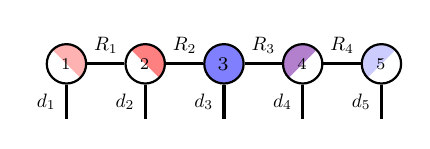
\begin{tikzpicture}[baseline=-0.5ex]
    \tikzset{tensor/.style = {minimum size = 0.5cm,shape = circle,thick,draw=black,inner sep = 0pt}, edge/.style = {thick,line width=.4mm},every loop/.style={}}
    \def\x{0}
    \def\y{0}
 \node[tensor, path picture={
        \fill[fill=red!30!white](path picture bounding box.south east)
        -- 
        (path picture bounding box.north west) --
        (path picture bounding box.north east) -- cycle;
        }, shift={(\x,\y)}] (A) {\scalebox{0.85}{$\At_1$}};
        \draw[edge](A) -- (\x,\y-0.7) node [midway,left] {\scalebox{0.7}{\dimcolor{$d_1$}}};
       \node[tensor, path picture={
        \fill[fill=red!50!white](path picture bounding box.south east)
        -- 
        (path picture bounding box.north west) --
        (path picture bounding box.north east) -- cycle;
        }, shift={(\x+1,\y)}] (B) {\scalebox{0.85}{$\At_2$}};
         \draw[edge](B) -- (\x+1,\y-0.7)node [midway,left] {\scalebox{0.7}{\dimcolor{$d_2$}}};
         \node[tensor,fill=blue!50!white] (C) at (\x+2,\y){$\At_3$};
          \draw[edge](C) -- (\x+2,\y-0.7)node [midway,left] {\scalebox{0.7}{\dimcolor{$d_3$}}};
          \node[tensor, path picture={
        \fill[fill=blue!60!red!50!](path picture bounding box.south west)
        -- 
        (path picture bounding box.north east) --
        (path picture bounding box.north west) -- cycle;
        }, shift={(\x+3,\y)}] (D) {\scalebox{0.85}{$\At_4$}};
         \draw[edge](D) -- (\x+3,\y-0.7)node [midway,left] {\scalebox{0.7}{\dimcolor{$d_4$}}};
        \node[tensor, path picture={
        \fill[fill=blue!20!white](path picture bounding box.south west)
        -- 
        (path picture bounding box.north east) --
        (path picture bounding box.north west) -- cycle;
        }, shift={(\x+4,\y)}] (E) {\scalebox{0.85}{$\At_5$}};
         \draw[edge](E) -- (\x+4,\y-0.7)node [midway,left] {\scalebox{0.7}{\dimcolor{$d_5$}}};
    \draw[edge](A) -- (B) node [midway,above] {\scalebox{0.7}{\dimcolor{$R_1$}}};
    \draw[edge](B) -- (C) node [midway,above] {\scalebox{0.7}{\dimcolor{$R_2$}}};
    \draw[edge](C) -- (D) node [midway,above] {\scalebox{0.7}{\dimcolor{$R_3$}}};
    \draw[edge](D) -- (E) node [midway,above] {\scalebox{0.7}{\dimcolor{$R_4$}}};
\end{tikzpicture}~~~\text{step:~3}
\caption{A half-sweep of TT-ALS}\label{fig:ortho-tt-als-alg}
\end{figure}
A half-sweep of TT-ALS is presented in Figure~\ref{fig:ortho-tt-als-alg}. In each non-QR step, the fully colored core is optimized, and in each QR step, the non-orthogonal component (depicted by a black circle)~is absorbed into the next core. This procedure repeats until reaching the right side of the decomposition, and then the same procedure is repeated from the right until reaching the left side (not demonstrated in this figure). The whole process is repeated until convergence. 
\begin{remark}
    This algorithm can be used with other loss functions in addition to the reconstruction error. In this case, the optimization of the loss w.r.t. one of the cores may not result in a least-squares problem, it is thus not called ALS anymore, but simply \emph{alternating minimization}. There also exists a two-site variant of this algorithm where pairs of consecutive cores are merged and optimized jointly at each iteration, before being split back in two using truncated SVD~\citep{holtz2012alternating}.
\end{remark}

